\section{Introduction}

With the development of neural networks, and their applications in industrial settings, the study of their reliability has become prevalent.
Many approaches have been studied to improve the trustworthiness of neural networks \cite{delseny2021whitepapermachinelearning}.
One of them is Uncertainty Quantification (UQ), which has become a key research domain for deploying safety-critical deep learning models. 
Its purpose is to provide additional information on the output of a model, indicating the confidence in its prediction.

We focus here on a UQ framework called Conformal Prediction (CP), which provides guarantees in nominal settings.
It is a finite-sample, distribution-free and model-agnostic framework that efficiently constructs prediction sets which contain the ground truth with high probability. 
The main underlying assumption is mild: calibration and test data points are assumed to be exchangeable (a lighter assumption than independence and identical distribution)~\cite{vovk}.
CP has successfully been applied to numerous fields: classification \cite{sadinle2019least, ding2024class}, regression \cite{papadopoulos2011regression, romano2019conformalized}, object detection \cite{andeol2023confident,timans2024adaptive}, semantic segmentation \cite{brunekreef2024kandinsky,mossina2024conformal} and generative models \cite{mohri2024language,teneggi2023trust}. 

Overall, CP represents a powerful tool in order to trust deep learning systems in their nominal settings.


\begin{figure*}[t!]
    \centering
    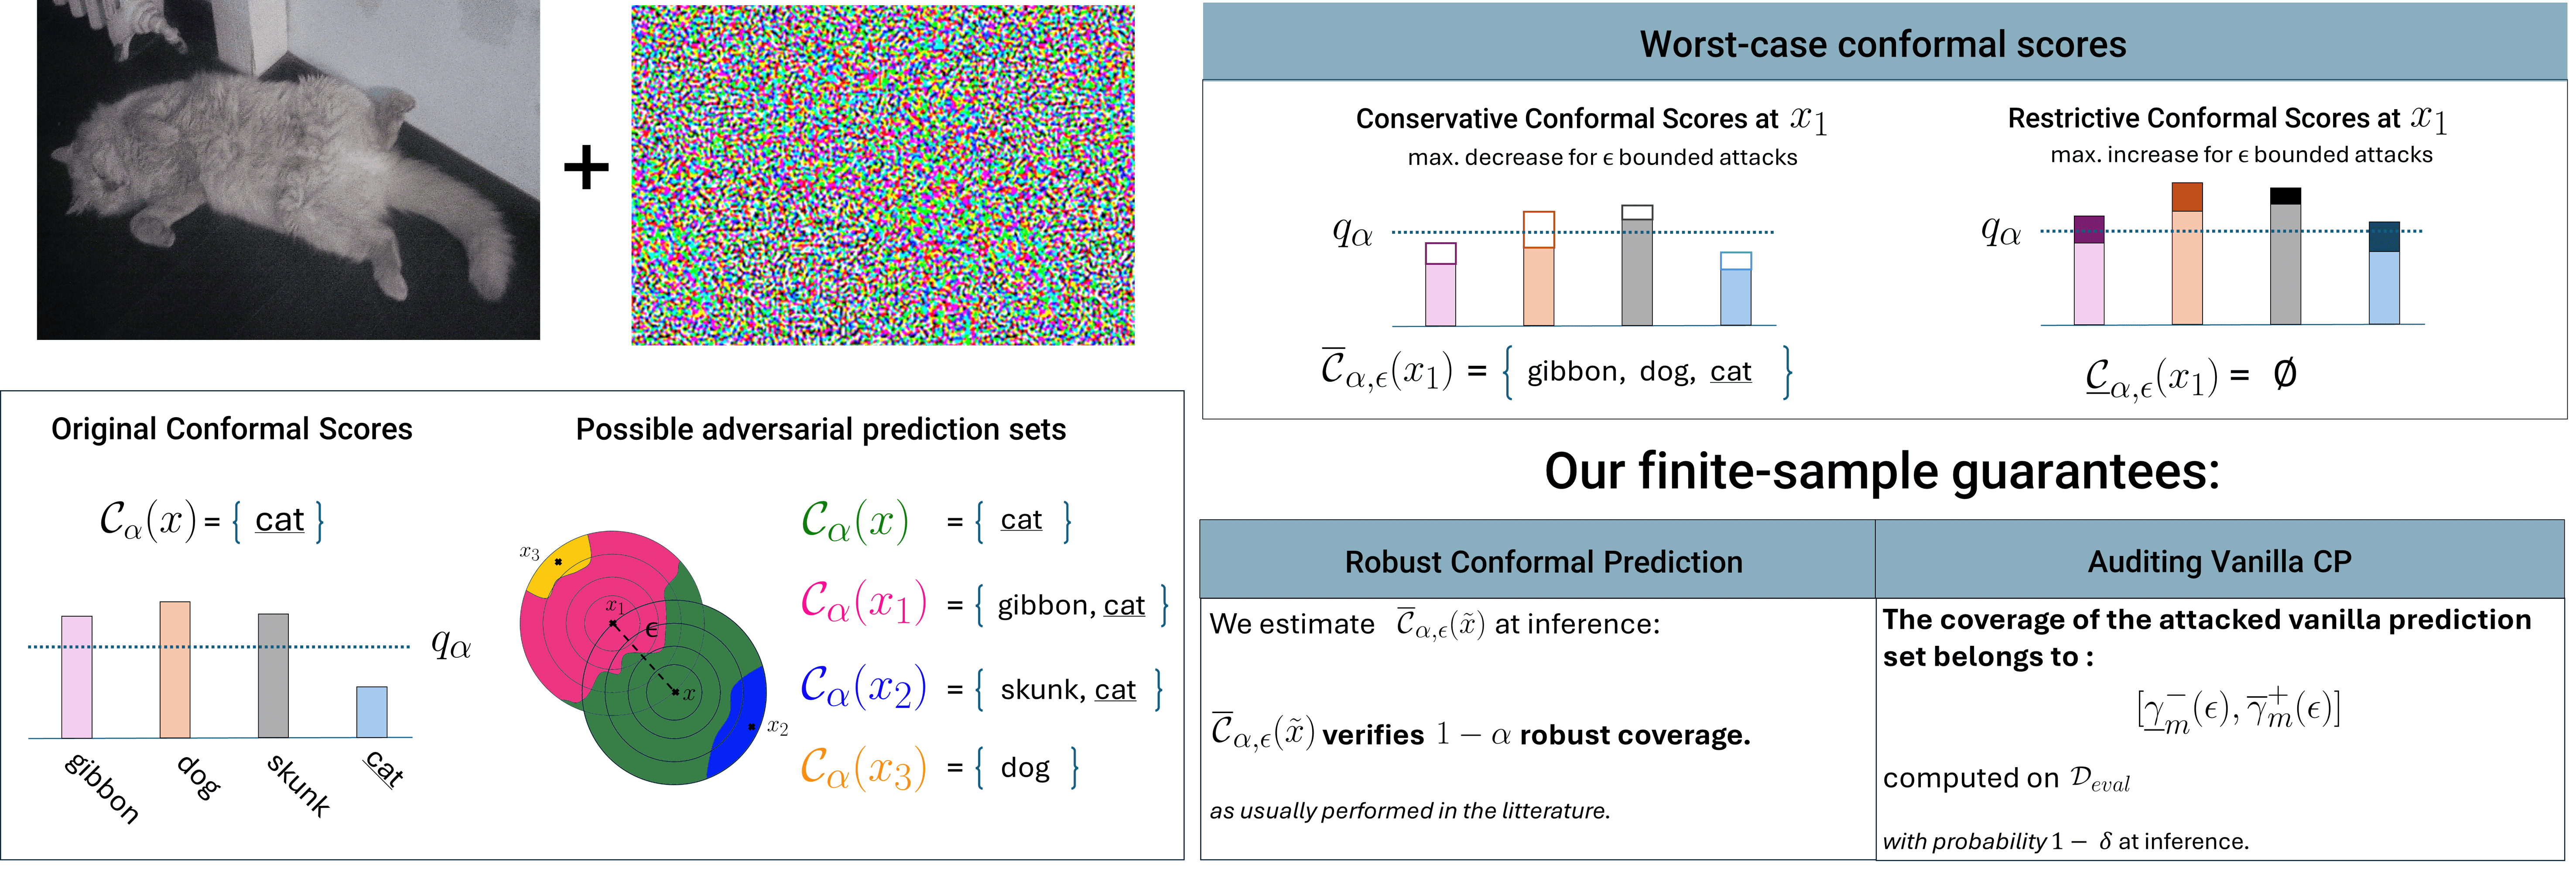
\includegraphics[width=0.9\linewidth]{banner_cat.png}
    \caption{
        Our framework allows different certifiable guarantees for conformal prediction sets. Through the fast estimation of worst-case conformal prediction scores, the user can either return 
        %the conservative prediction set 
        $\unionmetaset(\Tilde{x})$
        which provably verifies Def.~\ref{def:robust_coverage} 
        (\S ~\ref{sec:efficient_robust_sets}). Or, compute worst-case conformal coverage bounds $\covminmm(\epsilon)$ and $\covmaxmp(\epsilon)$ of vanilla CP sets on $\TestDataset$ through an efficient post-hoc auditing process on  a holdout dataset $\HoldoutDataset$. 
        This guarantee holds with probability $1 - \delta$ (\S~\ref{sec:vanillacoverage}). Importantly, the latter's coverage bounds hold over all $\epsilon$ levels.
    }
    \label{fig:cat_illustration}
\end{figure*}

However, research on adversarial robustness has demonstrated that state-of-the-art models can be misled with minimal adversarial input perturbations \cite{szegedy2014intriguingpropertiesneuralnetworks}.
This vulnerability has led to extensive research into adversarial robustness, focusing on both attack strategies and defense mechanisms \cite{goodfellow2015explainingharnessingadversarialexamples,carlini2017evaluatingrobustnessneuralnetworks}.

However, some popular adversarial defense strategies have been shown not to hold in the face of more sophisticated attacks \cite{athalye2018obfuscatedgradientsfalsesense}.
Therefore, research on certifiable robustness aims to provide theoretical worst-case guarantees for model performance under adversarial attacks independently from the attack method. 

These certified robustness methods also exhibit interesting properties in the domains of Reinforcement Learning \cite{liprl, formalverificationtrajectory}, Differential Privacy \cite{lipdp,wu2024augmentsmoothreconcilingdifferential}, explainable AI \cite{serrurier2024explainableproperties1lipschitzneural,Fel_2023_CVPR}.

\footnotetext{Throughout this paper we refer to standard CP as vanilla CP.}

\vspace{1cm} % forcing the line to the next page, otherwise the whole figure is clickable and a link to the reference Li et al.

Recently, some works in robust Conformal Prediction~\cite{li2024data,ledda2023adversarialattacksuncertaintyquantification,liu2024pitfallspromiseconformalinference} have demonstrated that minimal adversarial perturbations can undermine its associated guarantees.
Therefore, developing provably robust CP methods is a crucial objective in order to reconcile the guarantees of CP in nominal settings and the worst-case guarantees of certifiably robust systems.

Indeed, the vulnerability of CP methods to adversarial attacks raises significant concerns for deploying CP in safety-critical settings, where reliability is essential.

For this purpose, several approaches were proposed to construct robust conformal sets by using randomized smoothing methods~\cite{rscp,rscp_plus} or formal verification solvers~\cite{vrcp}. 
These methods inflate the CP sets in order for them to remain valid under adversarial conditions. 
Therefore, the performance of robust CP methods is measured by their ability to provide small and meaningful CP sets which maintain $1-\alpha$ conformal coverage under $\epsilon$-bounded perturbations.

Unfortunately, these works suffer from two penalties: they lack scalability, and/or provide conservative prediction sets that are too large for practical usage. We address these two shortcomings through the following set of contributions:

\begin{enumerate}
    \item We complement theoretical guarantees on robust CP from a different angle. We introduce a new method to audit vanilla CP's robustness to adversarial attacks. We derive the first sound coverage bounds for vanilla CP that are valid simultaneously across all attack levels.
    \item We provide a simple and efficient method, called \emph{lip-rcp}, to compute lower and upper bounds on CP scores under adversarial attacks. The method applies to any Lipschitz-bounded network, and can be used both to construct robust CP sets and to audit vanilla CP's robustness. It is tailored for efficiency and compatibility with real-time embedded systems.
    \item We propose to combine \emph{lip-rcp} with robust $1$-Lipschitz  networks with tight certified Lipschitz bounds. This allows to obtain tight estimates on worst-case variations of conformal prediction scores.
    \item We validate the whole approach across the \textsl{CIFAR-10}, \textsl{CIFAR-100}, \textsl{Tiny ImageNet} and \textsl{ImageNet} datasets. Our experiments showcase negligible computational overhead compared to vanilla CP, with best-in-class performances for both robust CP and vanilla CP's auditing.
\end{enumerate}
